\section{Class diagram}
%Introduktion til class diagrams

\begin{figure}[H]
	\centering
	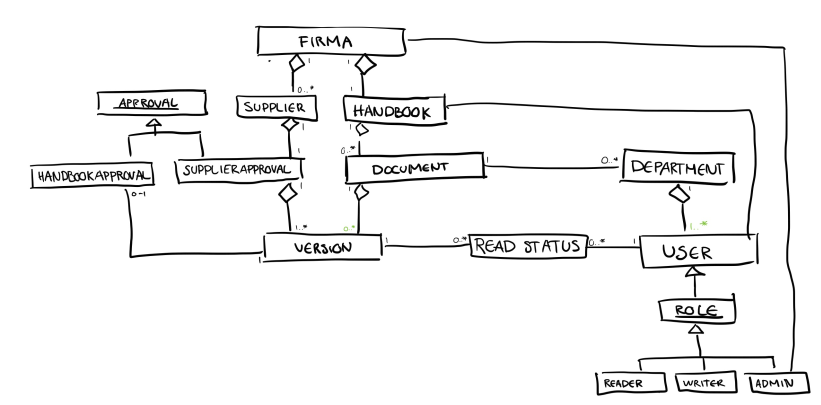
\includegraphics[width=0.95\textwidth]{billeder/classDiagram.png}
	\caption{\textit{Classdiagram of the problemdomain
	}}
	\label{fig:PACT-SystemImage}
\end{figure}

The system consists of two subsystems with similar functionalty:
The handbook subsystem and the supplier-approval subsystem.
Both subsystems archive and manage documents a company needs to get their certifications.

The handbook subsystem is the clients main concern and therefore the focus of the system. 
%Anna: Evt skrive "And will therefore after this analysis be the only one focused upon in the rest of the report"
In this system there is a Handbook aggregated by Document, as the Handbook exists to keep track of documents. The Document class is aggregated by version, which keeps track of the multiple versions each document has and when each one was valid in the handbook. Associated to Version is Approval since every single file in the handbook needs to have been approved, and it is necessary to keep track of who approved it and when.

The relation between Document and Version is an item-descriptor pattern. The Document class is the descriptor and contains all the important information about the document, including a pointer to the current valid version of said document. Version is an item as it encapsulates the actual file with the current version of Document. This is modeled so because of the need to keep track of earlier versions as well.

Version has two relational patterns, one to the Approval class and one to the Read Status class. Both classes exist because of the need to keep the information about when an event happened and which users were involved. Who approved this version and when did that happen? Who has read this version of the document? As well as the reverse: Who has not?

Document has a relation to Department. This is because a user should be shown relevant documents in the Handbook first as the book can become quite extensive but most users only need to access a couple documents regularly. A department connects a certain group of documents to a certain group of users. These departments are managed by an administrator of the system.

There are three different types of users in the system, which has been modeled by using a role pattern. The reader can read everything and verify that they have read a version of a document but nothing else. Every single user in the system has this level of access and it is therefore unnecessary to include as a class. However it is an important group and therefore, for the sake of clarity, it was included as a role nevertheless. The writer has the additional permission of submitting new versions of documents for approval while the administrator has all access to the system. It is expected that there will be between two and three administrators in the system. First the quality manager who will be the most accustomed to the system, second the secretary who has access for administrative purposes but usually will not work there much and possibly third the CEO of the company.

An important object for the user is the Table Of Contents (TOC). This table is needed to facilitate an overview of the documents, which is the point with the system. However this is not a class as its identity would be too similar to what is already included in the Handbook class. Besides that, because of the need for the TOC to be constantly updated the information this class would encapsulate would need to be recalculated each time someone accesses it anyway.
%var det her vores argumenter for at droppe klassen?
% Rasmus - Basically. Alt den information der var inkapsuleret i TOC klassen var allerede indkapsuleret i listen af dokumenter handbook havde, og derfor ville det være dobbeltkonfekt at have en TOC-klasse

The biggest similarities between the two subsystems are the need for archiving documents and the need for approving certain things with specified intervals.
The difference between them is first and foremost that the approval of the suppliers isn't actually included in the handbook and has no relevance for the majority of the users of this subsystem. Besides that the approval process for these systems vary slightly:
In the handbook system a version of a document needs to be approved by specified people.
In the supplier-approval system a supplier needs to be approved and only one person is needed to do that.
However that one person has to connect multiple documents that justify why the supplier has been approved.

Early versions of the class diagram modeled this association like in figure {\color{red}(whatevs)}. Here Supplier is aggregated by Approval as a Supplier will need to be reapproved after a certain time frame. Approval is again aggregated by Document as multiple files are submitted as documentation for the approval. In other words anyone can approve a supplier by submitting the appropriate documentation.

However in the handbook subsystem the Handbook is aggregated by Document and the
it is Version, the class that contains files, that needs to be approved and all the justification needed for an approval is the signature of



 which is modeled in the class diagram by having one common abstract superclass and a specialized subclass for each subsystem.
%still needed: Hændelser, event tabel, evt. kasserede klasser??? (har vi gemt dem???)
